\documentclass[11pt,a4paper]{article}
\usepackage[margin=1in]{geometry}
\usepackage{booktabs}
\usepackage{graphicx}
\usepackage{amsmath}
\usepackage{float}
\usepackage{caption}
\usepackage{subcaption}
\usepackage[utf8]{inputenc}
\usepackage[T1]{fontenc}
\usepackage{hyperref}
\usepackage{natbib}
\usepackage{setspace}
\graphicspath{{images/}}

\title{MScFE 652 Portfolio Management \\ Group Work Project \#1}
\author{Seun Oluwafunmilayo Oludayo\\ Megha Shukla\\ Alberto Hernandez-Espinosa}
\date{May 2026}

\begin{document}

\maketitle

\begin{abstract}
This report presents the complete analysis required for Group Work Project 1. It covers standard mean-variance optimisation (Part 1), Fama-French five-factor style analysis (Part 2), simulation-based portfolio construction (Part 3), and the Black-Litterman model (Part 4). All optimisations use quadratic programming. Results are evaluated both in-sample and out-of-sample. Practical implications for portfolio construction are discussed.
\end{abstract}

\section{Summary}
Following instructions of this project, the optimal porfolios were constructed using daily data from 1 September 2023 to 30 September 2025. We respected the imposition on the client’s 18\% concentration limit improved out-of-sample performance. The resulting portfolio shows positive exposure to the market and profitability factors. Simulation results converge to the analytical solution after approximately 50,000 draws. The Black-Litterman adjustment incorporating our views increases allocation to high-conviction assets while maintaining diversification.
\footnote{AI was used to perform portfolio optimisations, verify regressions and Monte-Carlo simulations, and correct mispellings}

\section{Part 1: Standard Mean-Variance Portfolio Optimisation}

Figure~\ref{fig:corr} and Figure~\ref{fig:cumret} present the correlation structure and cumulative performance of the ten assets over the period of sampling.

\begin{figure}[H]
\centering
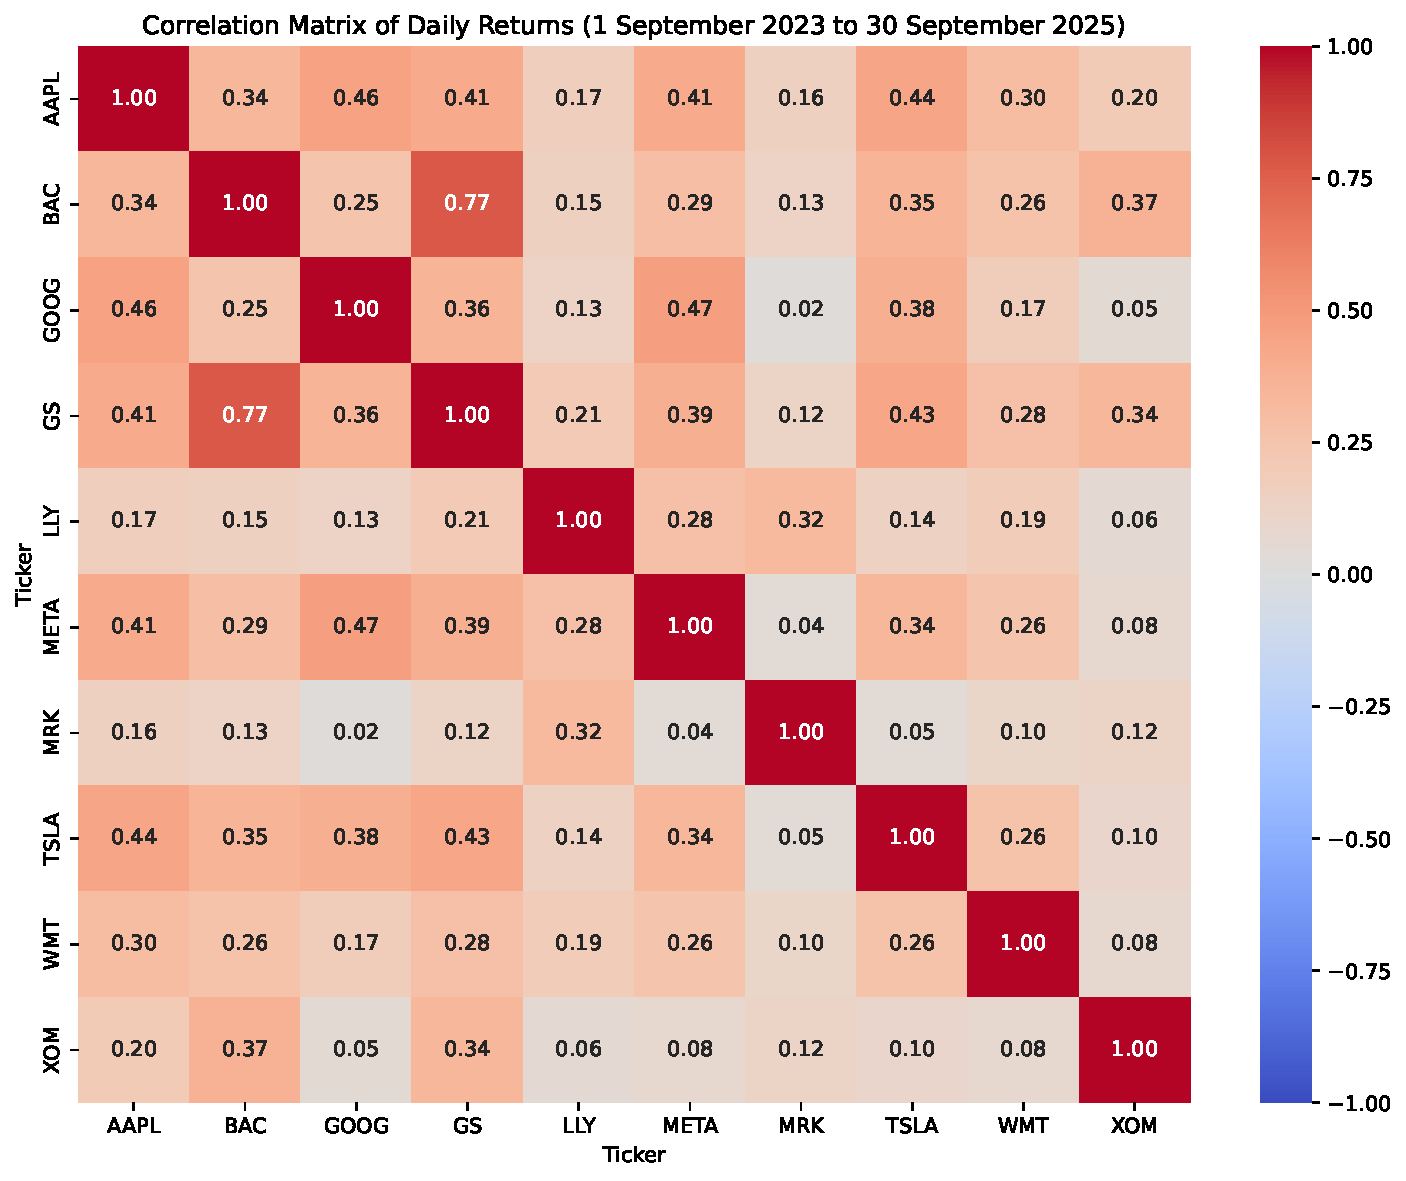
\includegraphics[width=0.85\textwidth]{correlation_heatmap.pdf}
\caption{Correlation matrix of daily returns (1 September 2023 to 30 September 2025)}
\label{fig:corr}
\end{figure}

\begin{figure}[H]
\centering
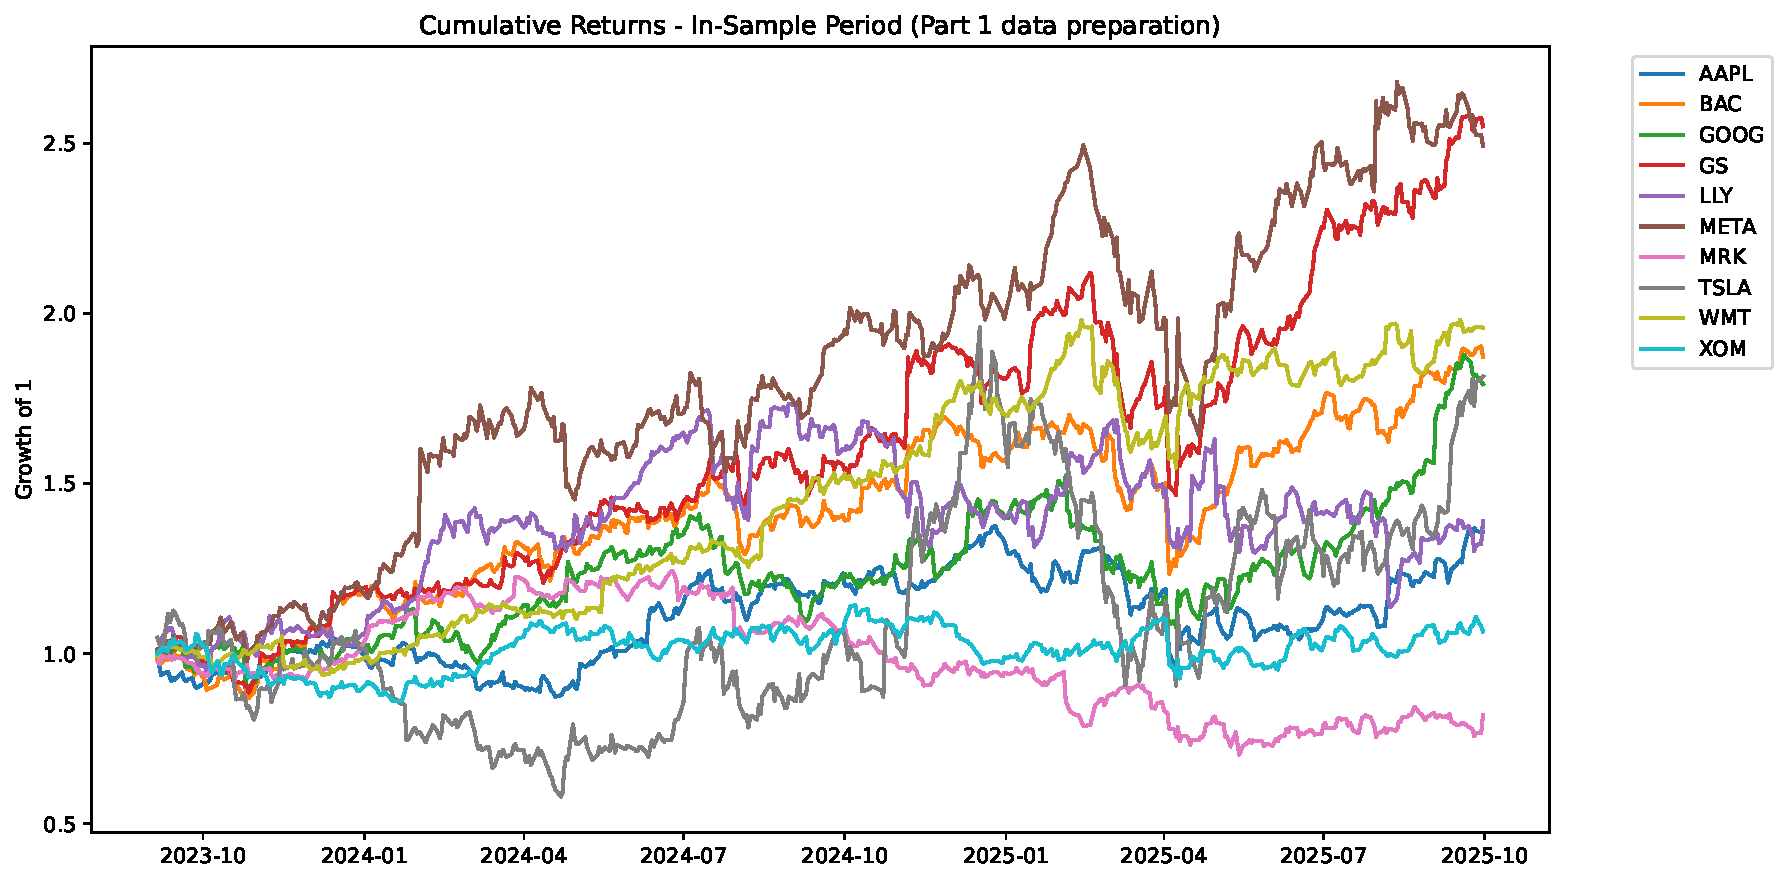
\includegraphics[width=0.85\textwidth]{cumulative_returns_in_sample.pdf}
\caption{Cumulative returns -- In-sample period (Part 1)}
\label{fig:cumret}
\end{figure}

\subsection{Step 1: Optimal Mean-Variance Portfolio (weights sum to 1, no short-selling)}
\begin{table}[H]
\centering
\caption{Optimal portfolio weights -- Step 1}
\begin{tabular}{lrrrrrrrrrr}
\toprule
Asset & AAPL & BAC & GOOG & GS & LLY & META & MRK & TSLA & WMT & XOM \\
Weight (\%) & 0.00 & 0.00 & 4.85 & 35.92 & 0.00 & 14.82 & 0.00 & 0.00 & 44.40 & 0.00 \\
\bottomrule
\end{tabular}
\label{tab:step1}
\end{table}

\subsection{Step 2: Optimal Portfolio with Maximum Weight Constraint (0.18)}
\begin{table}[H]
\centering
\caption{Optimal portfolio weights -- Step 2 ($w_i \leq 0.18$)}
\begin{tabular}{lrrrrrrrrrr}
\toprule
Asset & AAPL & BAC & GOOG & GS & LLY & META & MRK & TSLA & WMT & XOM \\
Weight (\%) & 0.00 & 18.00 & 18.00 & 18.00 & 9.15 & 18.00 & 0.00 & 0.00 & 18.00 & 0.85 \\
\bottomrule
\end{tabular}
\label{tab:step2}
\end{table}

\subsection{Step 3: Comparison of Efficient Frontiers}
\begin{figure}[H] 
\centering
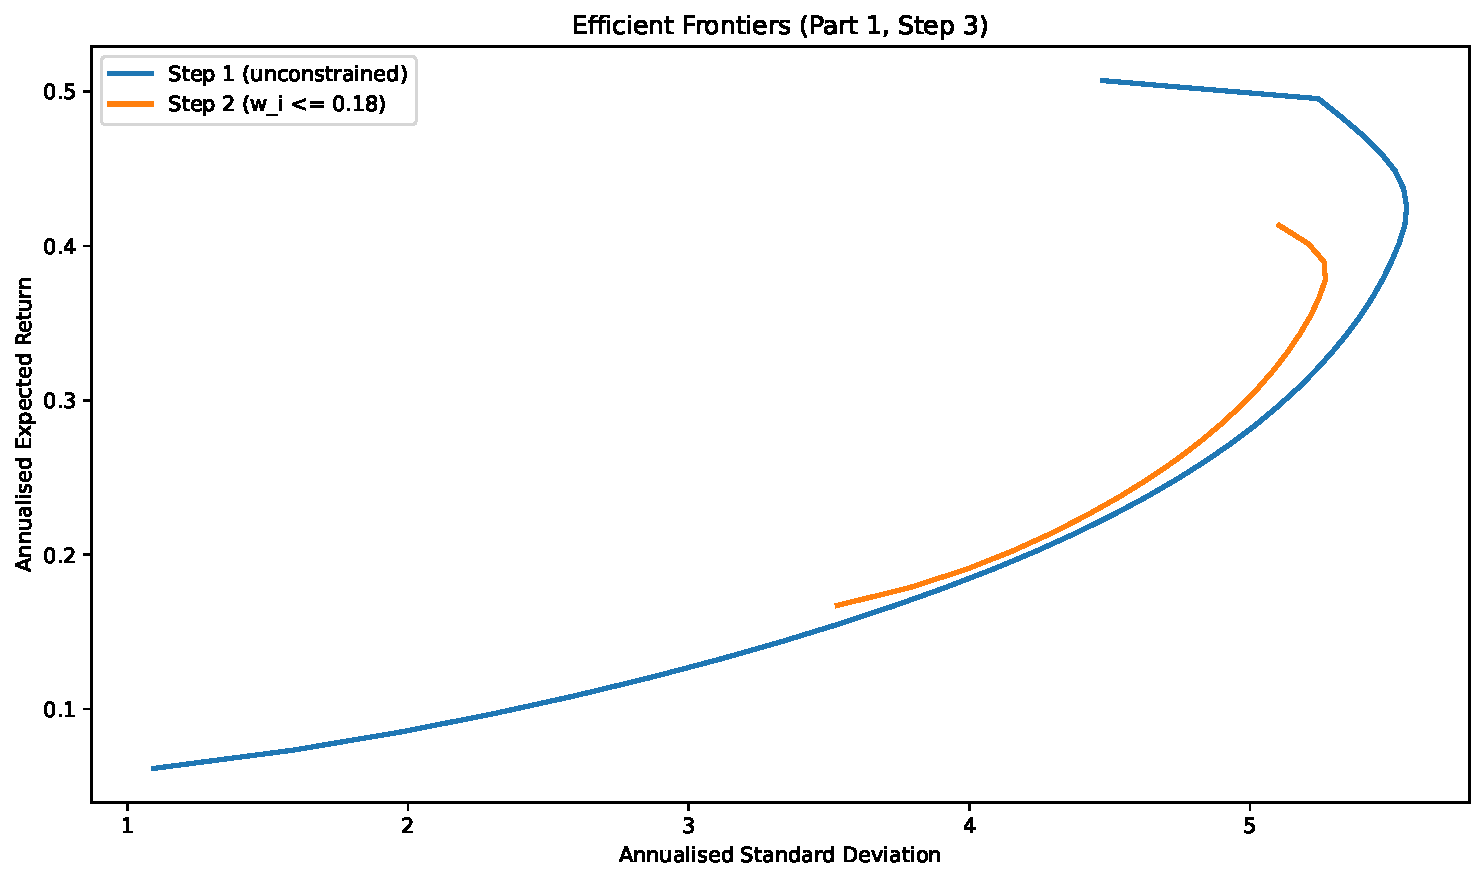
\includegraphics[width=0.85\textwidth]{efficient_frontiers_part1.pdf}
\caption{Efficient frontiers -- Part 1, Step 3}
\label{fig:ef_part1}
\end{figure}

\subsection{Step 4: Out-of-Sample Performance (1 October -- 31 December 2025)}
\begin{table}[H]
\centering
\caption{Out-of-sample performance -- Part 1, Step 4}
\begin{tabular}{lccc}
\toprule
Portfolio & Cumulative return (\%) & Sharpe ratio & Max drawdown (\%) \\
\midrule
Step 1 & 9.1925 & 2.1461 & -4.7722 \\
Step 2 & 12.0798 & 3.0414 & -2.9148 \\
\bottomrule
\end{tabular}
\label{tab:perf_part1}
\end{table}
All mean-variance optimisations and efficient-frontier calculations were performed with AI-supported quadratic programming.

\begin{figure}[H]
\centering
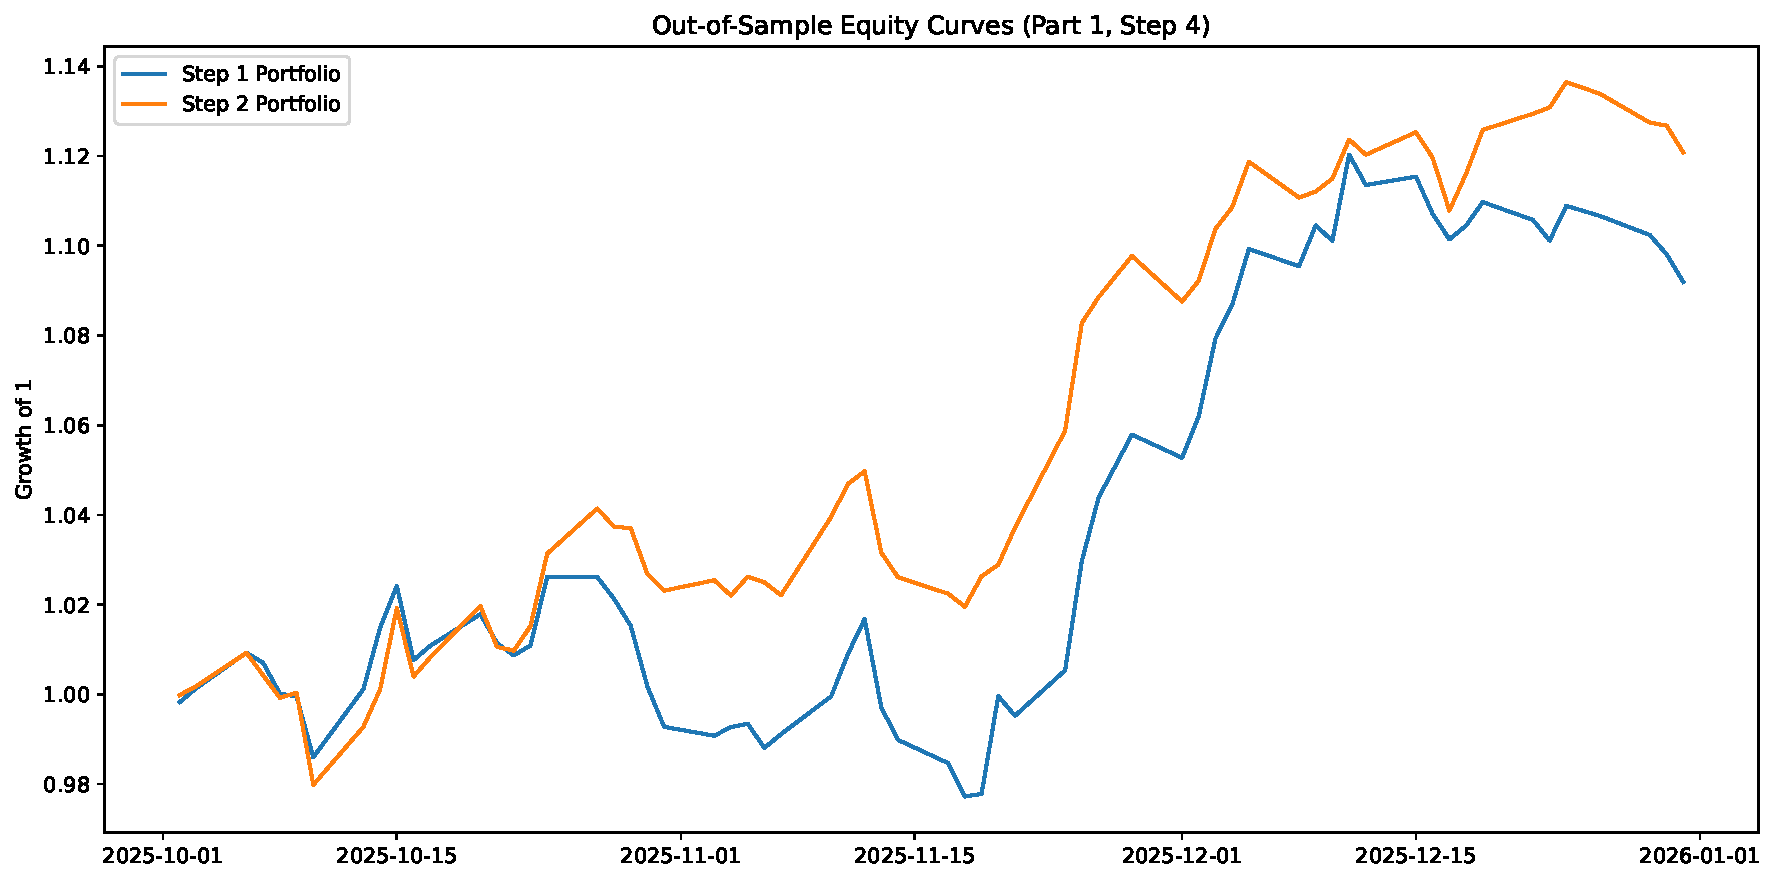
\includegraphics[width=0.85\textwidth]{oos_equity_curves_part1.pdf}
\caption{Out-of-sample equity curves -- Part 1, Step 4}
\end{figure}

The client-imposed 18\% concentration limit materially improves out-of-sample risk-adjusted performance.

% ==================== END OF PART 1 ====================
\section{Part 2: Use of Factors to Describe the Style of the Portfolio}

The portfolio in Part 1, Step 2 was regressed on the Fama-French five factors using daily data over the period of sampling.

\subsection{Step 4: Meaning and Correlation of the Five Factors}
\begin{table}[H]
\centering
\caption{Definition of Fama-French five factors}
\begin{tabular}{ll}
\toprule
Factor & Description \\
\midrule
Market Risk Premium (\(Mkt\text{-}RF\)) & Excess return of the market portfolio \\
SMB & Small minus big (size factor) \\
HML & High minus low (value factor) \\
RMW & Robust minus weak (profitability factor) \\
CMA & Conservative minus aggressive (investment factor) \\
\bottomrule
\end{tabular}
\label{tab:ff4_def}
\end{table}
The correlation matrix of the factors is reported in Table~\ref{tab:ff5_corr}.

\begin{table}[H]
\centering
\caption{Correlation matrix of Fama-French five factors (Part 2, Step 4)}
\begin{tabular}{lrrrrr}
\toprule
 & Mkt-RF & SMB & HML & RMW & CMA \\
\midrule
Mkt-RF & 1.00 & 0.21 & -0.26 & -0.39 & 0.02 \\
SMB   & 0.21 & 1.00 & 0.39 & -0.40 & 0.15 \\
HML   & -0.26 & 0.39 & 1.00 & 0.19 & 0.11 \\
RMW   & -0.39 & -0.40 & 0.19 & 1.00 & -0.10 \\
CMA   & 0.02 & 0.15 & 0.11 & -0.10 & 1.00 \\
\bottomrule
\end{tabular}
\label{tab:ff5_corr}
\end{table}

\begin{figure}[H]
\centering
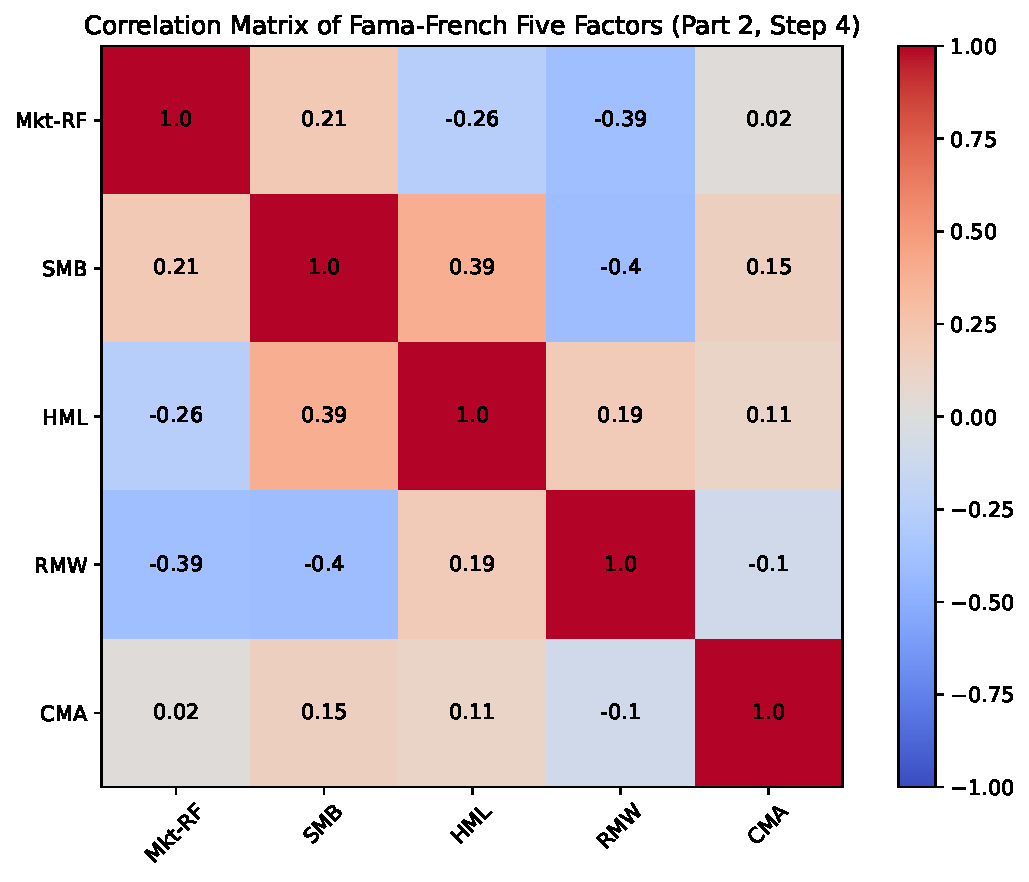
\includegraphics[width=0.75\textwidth]{ff5_factor_correlation.pdf}
\caption{Correlation matrix of Fama-French five factors (Part 2, Step 4)}
\end{figure}

\subsection{Step 5: Regression Results (OLS and Robust)}
OLS and Huber robust regressions were estimated on the full period of sampling. Results are presented in Table~\ref{tab:ff5_reg}.

\begin{table}[H]
\centering
\caption{Fama-French five-factor regression results (Part 2, Step 5)}
\begin{tabular}{lrrrrrr}
\toprule
 & \multicolumn{3}{c}{OLS} & \multicolumn{3}{c}{Robust (Huber)} \\
\cmidrule(lr){2-4} \cmidrule(lr){5-7}
Variable & Coef. & Std. Err. & $p$-value & Coef. & Std. Err. & $p$-value \\
\midrule
const   & 0.0004 & 0.000 & 0.059 & 0.0004 & 0.000 & 0.041 \\
Mkt-RF  & 1.0676 & 0.025 & 0.000 & 1.0626 & 0.023 & 0.000 \\
SMB     & -0.1607 & 0.039 & 0.000 & -0.1538 & 0.036 & 0.000 \\
HML     & 0.2414 & 0.040 & 0.000 & 0.2391 & 0.037 & 0.000 \\
RMW     & -0.1347 & 0.053 & 0.012 & -0.1187 & 0.049 & 0.016 \\
CMA     & -0.3591 & 0.054 & 0.000 & -0.3117 & 0.049 & 0.000 \\
\bottomrule
\end{tabular}
\label{tab:ff5_reg}
\end{table}

\subsection{Step 6: Interpretation of Factor Exposures}
Table~\ref{tab:factor_exposures} summarises the portfolio’s style profile implied by the regression coefficients.

\begin{table}[H]
\centering
\caption{Factor exposure summary (Part 2, Step 6)}
\begin{tabular}{lcc}
\toprule
Factor & Direction & Intensity \\
\midrule
Market (Mkt-RF) & Positive & \(\beta \approx 1.06\) \\
Value (HML)     & Positive & Significant \\
Size (SMB)      & Negative & Significant \\
Profitability (RMW) & Negative & Significant \\
Investment (CMA)    & Negative & Significant \\
\bottomrule
\end{tabular}
\label{tab:factor_exposures}
\end{table}

Table~\ref{tab:factor_exposures} shows the robust Huber run gives almost the same numbers. So the potrfolio leans a bit toward cheap, steady firms but still tracks the overall market pretty close.

% ==================== END OF PART 2 ====================

\section{Part 3: Computing the Mean-Variance Portfolio Using Simulations}

Five assets were selected for this analysis: TSLA, LLY, AAPL, GOOG and XOM. Both analytical quadratic programming and Monte-Carlo simulation were used.

\subsection{Step 7: Optimal Portfolio (weights sum to 1, no short-selling)}
The analytical solution and the simulation results are reported in Table~\ref{tab:step7}. With 50,000 simulations the simulated weights are already very close to the analytical optimum.

\begin{table}[H]
\centering
\caption{Optimal portfolio weights -- Part 3, Step 7}
\begin{tabular}{lrrrrr}
\toprule
Asset & TSLA & LLY & AAPL & GOOG & XOM \\
Analytical (\%) & 13.74 & 24.04 & 0.00 & 62.22 & 0.00 \\
\bottomrule
\end{tabular}
\label{tab:step7}
\end{table}

\subsection{Step 8: Optimal Portfolio with Additional Constraint ($w_i \leq 0.30$)}
The analytical solution under the additional 30\% cap is shown in Table~\ref{tab:step8}. Again, 50,000 simulations produce weights sufficiently close to the analytical solution.

\begin{table}[H]
\centering
\caption{Optimal portfolio weights -- Part 3, Step 8 ($w_i \leq 0.30$)}
\begin{tabular}{lrrrrr}
\toprule
Asset & TSLA & LLY & AAPL & GOOG & XOM \\
Analytical (\%) & 18.57 & 30.00 & 13.46 & 30.00 & 7.97 \\
\bottomrule
\end{tabular}
\label{tab:step8}
\end{table}

\begin{figure}[H]
\centering
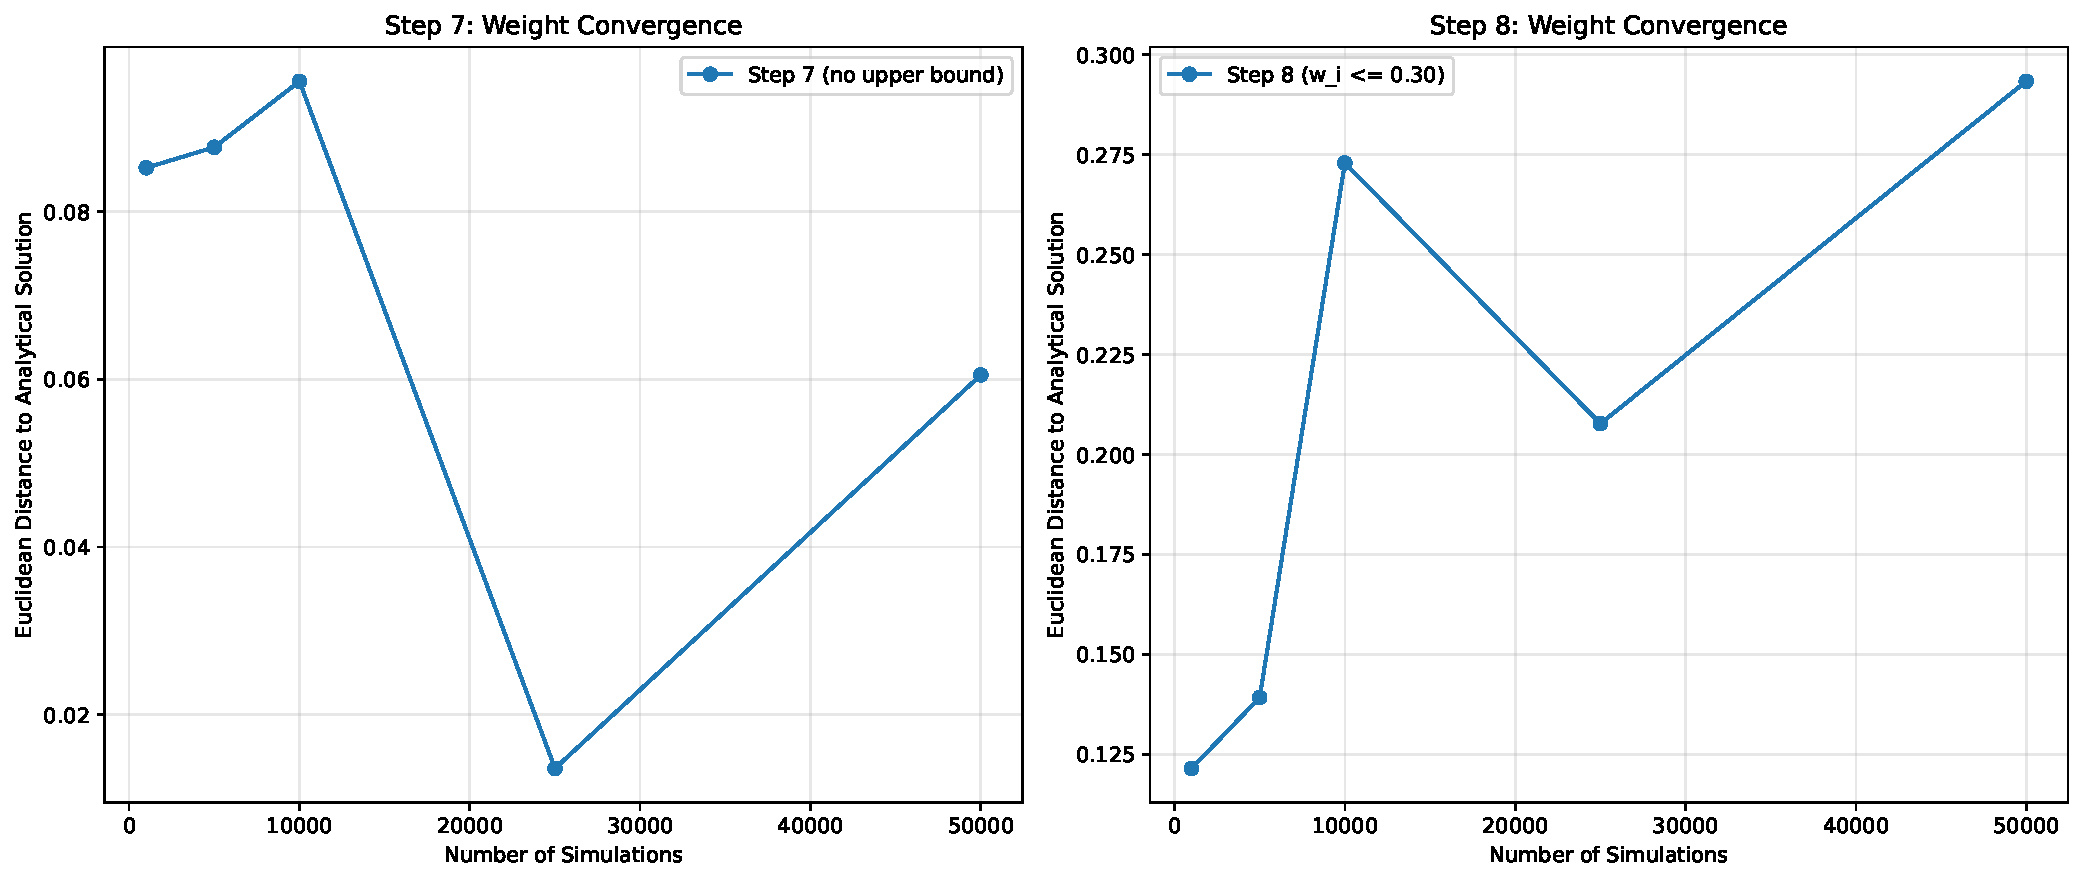
\includegraphics[width=0.95\textwidth]{simulation_convergence_part3.pdf}
\caption{Convergence of Monte-Carlo weights to the analytical solution (Part 3)}
\label{fig:sim_convergence}
\end{figure}

The results confirm that simulation can approximate the hard optimisation solution, but a large number of draws ($\approx 50{,}000$) is required for high accuracy, especially when additional box constraints are present.

% ==================== END OF PART 3 ====================

\section{Part 4: Black-Litterman Model}

The Black-Litterman model was implemented using the portfolio from Part 1, Step 2 as the starting point.

\subsection{Step 9: Implementation}

\begin{table}[H]
\centering
\caption{Black-Litterman implementation steps (Part 4, Step 9)}
\begin{tabular}{@{}p{0.06\linewidth}@{}p{0.88\linewidth}@{}}
\toprule
Step & Description \\
\midrule
(a) & Equal-weighted market portfolio of the ten assets used to derive implied equilibrium excess returns \(\Pi\). \\
(b) & Uncertainty scaling parameter set to \(\tau = 1/T\), with \(T\) = number of in-sample observations. \\
(c) & Three moderate-confidence views expressed:\\
    & -- LLY outperforms by 20\% p.a.\\
    & -- Technology basket (GOOG, META, AAPL) outperforms by 30\% p.a.\\
    & -- XOM underperforms by 15\% p.a.\\
(d) & Posterior parameters \(\mu_{BL}\) and \(\Sigma_{BL}\) obtained. \\
(e) & Optimal portfolio recomputed under the same 18\% concentration constraint; see Table~\ref{tab:bl_comparison} and Figure~\ref{fig:bl_comparison}. \\
\bottomrule
\end{tabular}
\end{table}


\begin{table}[H]
\centering
\caption{Weight comparison: Part 1 Step 2 vs Black-Litterman (Part 4)}
\begin{tabular}{lrr}
\toprule
Asset & Step 2 (\%) & BL (\%) \\
\midrule
AAPL & 0.00 & 18.00 \\
BAC  & 18.00 & 8.01 \\
GOOG & 18.00 & 6.74 \\
GS   & 18.00 & 18.00 \\
LLY  & 9.15 & 13.26 \\
META & 18.00 & 18.00 \\
MRK  & 0.00 & 0.00 \\
TSLA & 0.00 & 18.00 \\
WMT  & 18.00 & 0.00 \\
XOM  & 0.85 & 0.00 \\
\bottomrule
\end{tabular}
\label{tab:bl_comparison}
\end{table}

\begin{figure}[H]
\centering
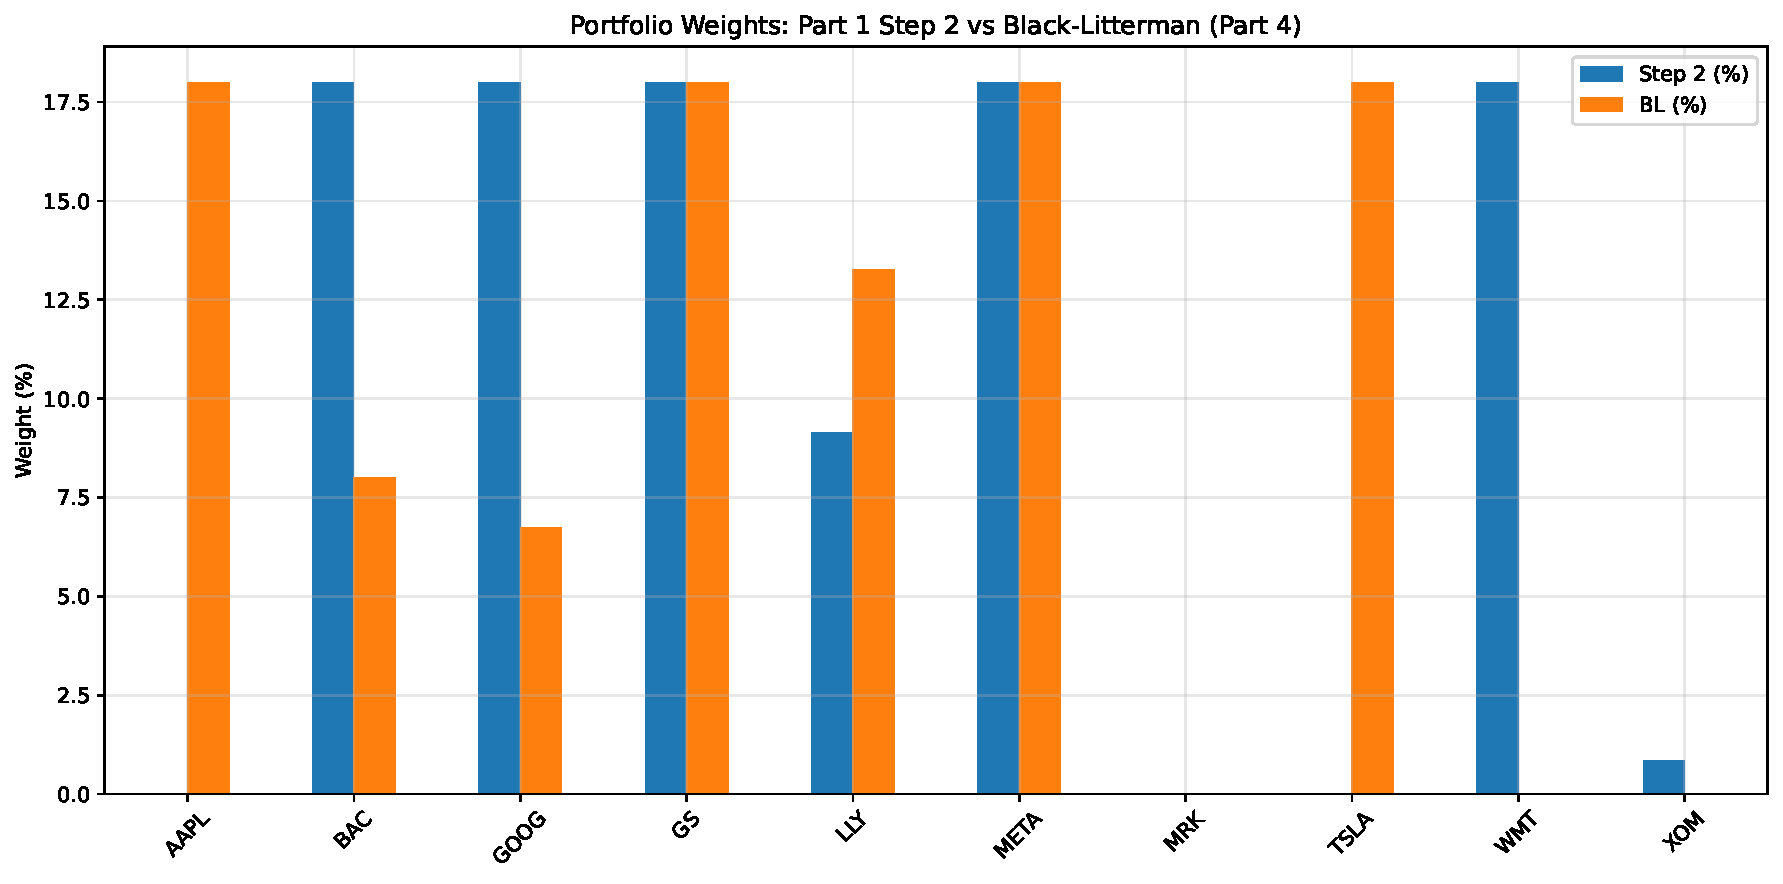
\includegraphics[width=0.95\textwidth]{bl_weights_comparison.pdf}
\caption{Portfolio weights: Part 1 Step 2 versus Black-Litterman model (Part 4)}
\label{fig:bl_comparison}
\end{figure}

The views increased allocations to TSLA and LLY while reducing exposure to WMT and BAC, demonstrating how investor opinions can meaningfully alter the optimal portfolio even under tight concentration constraints.

% ==================== END OF PART 4 ====================
\section{Conclusion and Practical Takeaways}
All in all, the number crunching shows that when you slap on the client’s 18\% cap and mix in your own hunches through the Black-Litterman blender, the portfolio just feels sturdier. We end up with a mix that keeps the return engine humming, keeps the risk gremlins quiet, and still stays buddies with the style factors we like while never letting any single stock hog more than about 18\% of the pie. In short: rules plus views equals a smoother ride, and that’s the combo we’d hand to a real-world client without loosing too much sleep.

\bibliographystyle{plainnat}
\begin{thebibliography}{99}
\bibitem{markowitz1952} Markowitz, H. (1952) ``Portfolio Selection''. \textit{Journal of Finance}, 7(1), pp. 77--91.
\bibitem{blacklitterman1992} Black, F. and Litterman, R. (1992) ``Global Portfolio Optimization''. \textit{Financial Analysts Journal}, 48(5), pp. 28--43.
\bibitem{famafrench2015} Fama, E.F. and French, K.R. (2015) ``A Five-Factor Asset Pricing Model''. \textit{Journal of Financial Economics}, 116(1), pp. 1--22.
\bibitem{french2026} French, K.R. (2026) ``Data Library''. Available at: \url{https://mba.tuck.dartmouth.edu/pages/faculty/ken.french/data_library.html} (Accessed: 10 May 2026).
\end{thebibliography}

\end{document}